\documentclass[a4paper,oneside,11pt]{scrreprt}
\usepackage{scrhack} % to suppress warning

% include style from other file
\usepackage{style}

\begin{document}

\pagenumbering{gobble}

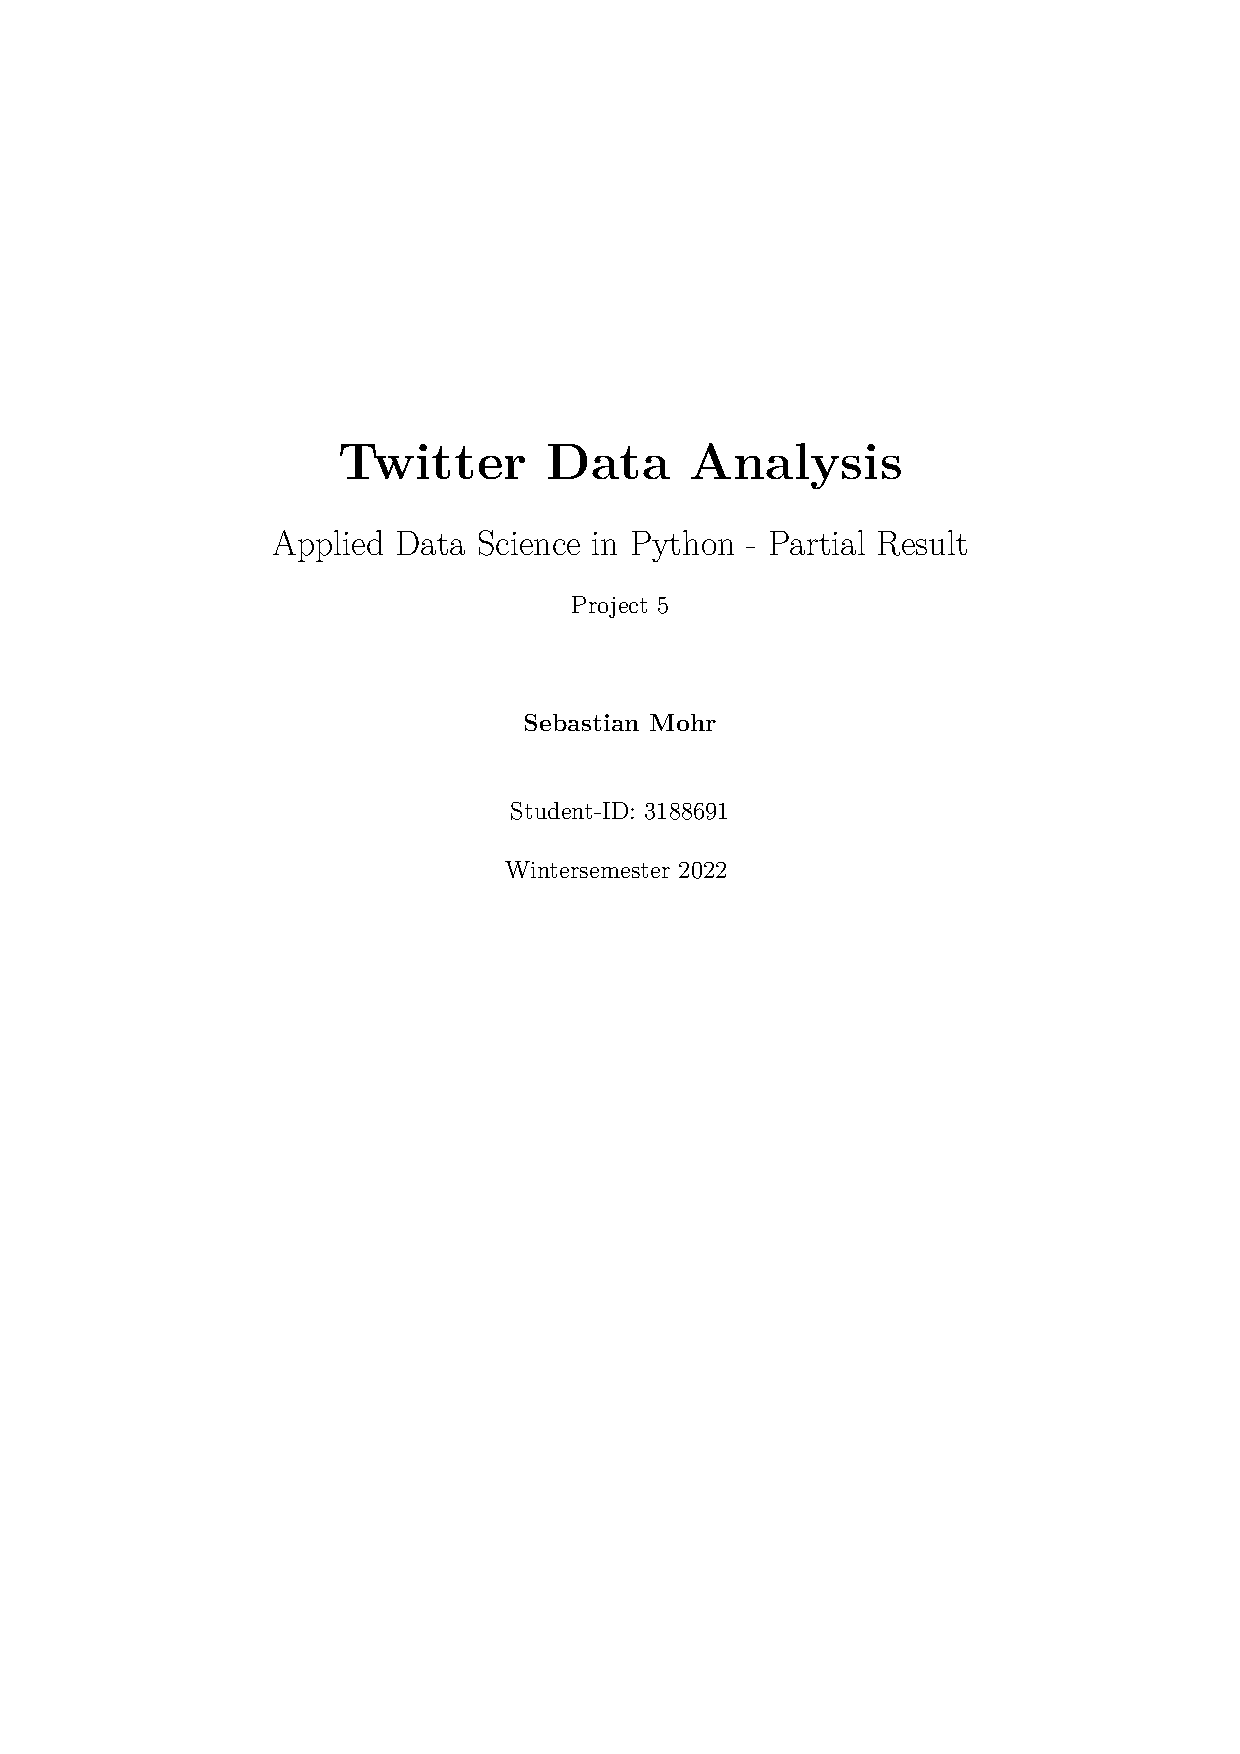
\includepdf{cover.pdf}

\newpage

\pagenumbering{arabic}

\chapter{Loading in of data}

The data will be loaded through the Twitter API. The easiest way for this is to use the Python library \code{Tweepy} that provides different methods to access the Twitter API. The first step here will be the input of a specific events hashtag, for example the current Fifa World Cup 2022 uses the official Hashtag \requirement{\#FIFAWorldCup}. After the tag has been put into the application, it will request a specific number of tweets for this event from the Twitter API. Currently I go with 50 tweets, but this number can be also set higher or lower, depending on preferences on how detailed the analyzed data should be. \\

To load the data, a \requirement{URL} has to be defined, which accesses the API at a specific endpoint. The URL also defines the query parameters, such as how many tweets are requested, which hashtags should be included in each tweet or which timeframe the tweet has to be created in. In \code{Tweepy} this process is done by creating a \code{Tweepy} Client, that includes the Bearer Token, through which the Twitter API can authenticate the current used dev-User. The defined query parameters then get put into the \code{client.search\_recent\_tweets(...)} method, that then starts an API call and retrieves all matching tweets. This method also takes in the definition of which fields of the tweets are necessary and will be be included in the result. The data will then be stored in a CSV file to make it easily accessable in a later session.


\chapter{Sentiment Analysis}

After the tweets have been loaded into the application, they have to be analyzed to show them to the user. For this part of the project I will use the Python library \code{Textblob} that is specialized on natural language processing.


\begin{figure}[h]
    \centering
    \caption{Flowchart of the sentiment analysis}
    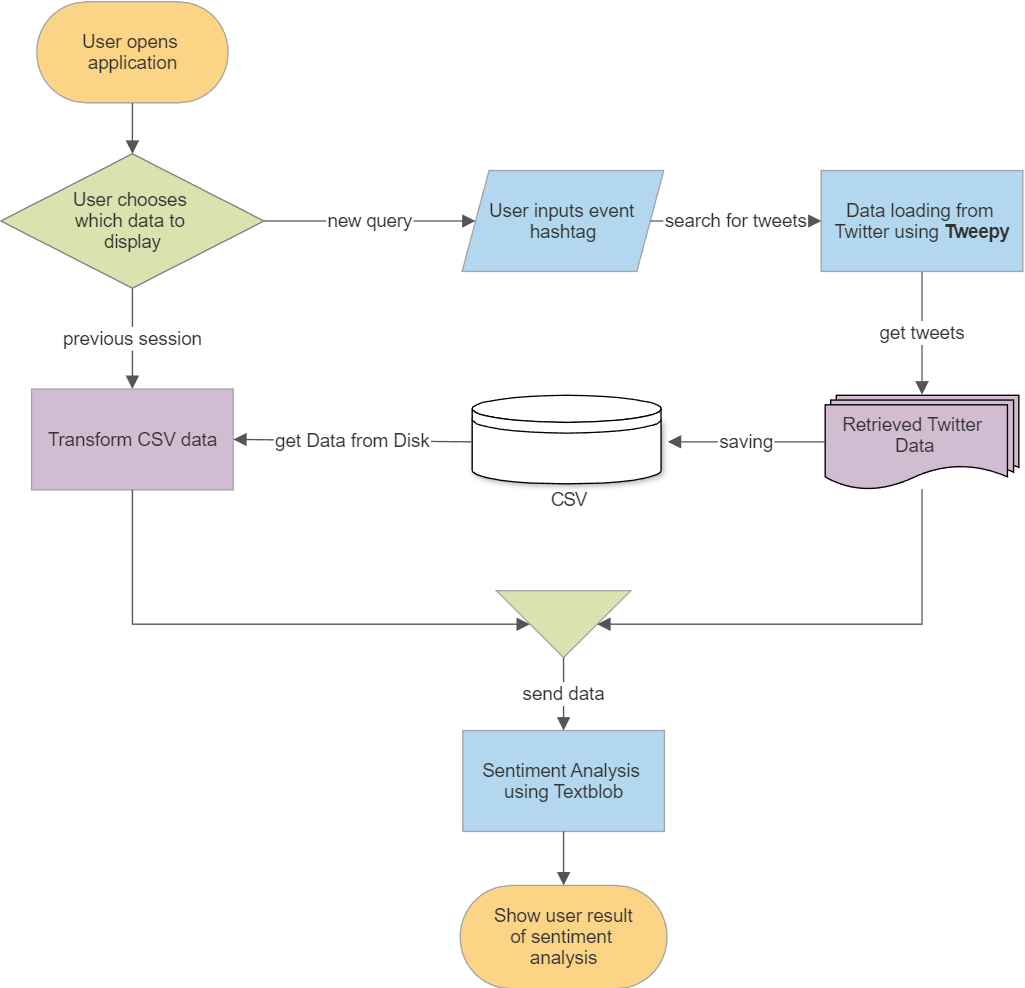
\includegraphics[width=0.95\textwidth]{media/sentiment_analysis_flowchart.png}
\end{figure}

After the user opens the application, they can choose to either start a new query by inputting a new hashtag or to view the previous session. When choosing the previous session, the stored data from the CSV will be loaded and transformed into a python object. When a new query is started, the application will load the data from twitter using \code{Tweepy}. After the data is ready, it gets sent into the sentiment analysis, that gets done through using \code{Textblob}. Afterwards the result gets displayed to the user.


\chapter{Solution Examples}
At the time of this submission the application is not yet up and running. So the following examples will just be some mockups, on how the data will be displayed to the user after it was analyzed. 

\end{document}